\section{Calculus of variations}
\label{sec:calculus-of-variations}

\subsection{Functionals}

In the calculus of variations, we compute the extrema of a possibly nonlinear 
\emph{function of a function}. Such objects are often called
\emph{functionals}. Thus, a functional $F[u]$ takes some \emph{function}
$u$ and produces a \emph{number}. One can think of $F$ depending on
infinitude of function values $u(x)$. In the case of the energy expectation
value, the $N$-body wavefunction $\ket{\Psi}$ is mapped to the number
\[ \mathcal{E}[\ket{\Psi}] =
\braket{\Psi|\hat{H}|\Psi}/\braket{\Psi|\Psi}. \] 
Suppose we expand the wavefunction in a basis, say, a Slater
determinant basis,
\[ \ket{\Psi} = \sum_I A_I \ket{\Phi_I}.\]
Then, $\mathcal{E}$ becomes a function of the vector $\vec{A}$, a
possibly infinite set of coefficients. This may be an easier way to
think of a functional: a function that depends on $K$ variables, where
$K$ may be infinite.

A functional can also depend on more than one function. In
Hartree--Fock theory, the energy functional depends on $N$
single-particle functions $\phi_i$, $i=1,\cdots,N$. Moreover, the
Hartree--Fock Lagrangian function that we \emph{actually} optimize is
a functional that also depends on a matrix $\lambda=[\lambda_{ij}]$ of
Lagrange multipliers, $\mathcal{L} =
\mathcal{L}[\phi_1,\cdots,\phi_N,\lambda]$. Given expansions of the
$\phi_i$ as $\phi_i(x) = \sum_p \chi_p(x) U_{ip}$, we see that
$\mathcal{L}$ becomes a function of the matrix $U$ and the matrix
$\lambda$. Thus, functionals are not too different from ordinary
functions of a vectors.

How do we go about computing the extrema of a functional?  A function
of a single real variable has an intuitive notion of a local extremum,
and most readers probably have an intuitive notion of extrema of
two-variable functions as well. But if we go to higher dimensions (or
infinite dimensions!)  it becomes more complicated.

We will therefore introduce the concept of a \emph{directional
  derivative} in a rather informal way. This is very handy, and allows
us to read off the condition for an extremum in a straight-forward
manner. This framework is called \emph{the calculus of variations},
since we are computing the ``variation in $F[u]$'' with respect to
arbitrary ``variations $\delta u$ of the function $u$''.

\subsection{Functions of one real variable}

Consider first a simple
function $F : I \to \RR$, $I\subset \RR$ being an interval. Suppose
$x_0 \in I$. Assuming that $F$ can be differentiated at leat twice, we can compute
a second-order Taylor expansion around $x_0$, viz,
\begin{equation}
  F(x_0 + \epsilon) \approx  F(x_0) + \epsilon F'(x_0) +
  \frac{1}{2}\epsilon^2 F''(x_0) .
\end{equation}
The error in this approximation vanishes as $\epsilon\to 0$.

The condition for an extremum at $x_0$ is $F'(x_0)=0$. The
second-order term tells us the nature of the extremum: 
if $F''(x_0) > 0$ then $x_0$ is a local minimum. If $F''(x_0) < 0$
then $x_0$ is a local maximum. Finally, if $F''(x_0) = 0$, we cannot
determine right away if we have a maximum or minimum. We may have
neither, as for $F(x) = x^3$, where $x_0 = 0$ is a saddle point. A
minimum and a saddle point is illustrated in Fig.~\ref{fig:extrema-1}.

\begin{figure}
  \begin{center}

    \begin{tikzpicture}
      \begin{scope}[xshift=0cm]
        \draw[->] (-2,0) -- (2,0) node[right] {$x$};
        \draw[->] (0,0) -- (0,4) node[above] {$F(x)$};
        \draw[scale=1.0,domain=-2:2,smooth,variable=\x,blue] plot
        ({\x},{\x*\x});
        \filldraw (0,0) circle (.1) node[anchor=north] {$x_0$};  
      \end{scope}
      \begin{scope}[xshift=5cm]
        \draw[->] (-2,0) -- (2,0) node[right] {$x$};
        \draw[->] (0,0) -- (0,4) node[above] {$F(x)$};
        \draw[scale=1.0,domain=-2:2,smooth,variable=\x,blue] plot
        ({\x},{10*\x*\x*sin(\x)});
        \filldraw (0,0) circle (.1) node[anchor=north] {$x_0$};  
      \end{scope}
    \end{tikzpicture}

    \caption{Simple functions of one real variables with a local
      minimum ($F''(x_0)>0$) (left) and a saddle point ($F''(x_0) =
      0$) (right).\label{fig:extrema-1}.}
  \end{center}
\end{figure}


\subsection{Functions of two real variables}

Consider yourself in a landscape of mountains and valleys. The
elevation is $F(x,y)$. You are trying to find, say, a local minimum
$(x_0,y_0)$ of elevation. On a map, a local minimum will show up as
successively smaller closed curves of equal elevation, see
Fig.~\ref{fig:extrema-2}. (The same is true for a maximum, and a saddle
point is a crossing of lines of equal elevation.) We now observe, that
if you move in a direction $\eta = (\delta x, \delta y) \neq 0$ from the
local minium, you
\emph{will always walk uphill}, that is, the function
\[ f(\epsilon) = F(x_0 + \epsilon \delta x, y_0 + \epsilon \delta
y) \]
has a local minimum at $\epsilon=0$, irrespective of $\eta$.
If you were standing on a mountaintop (a local maximum) you
would always walk downhill, and $f(\epsilon)$ would always have a
local maximum at $\epsilon=0$. 

\begin{figure}
  \begin{center}
    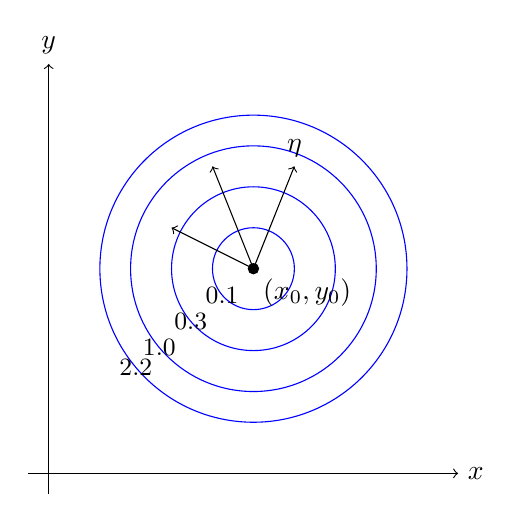
\begin{tikzpicture}[scale=1.3]
      \draw[->] (-.2,0) -- (4,0) node[anchor=west] {$x$};
      \draw[->] (0,-.2) -- (0,4) node[anchor=south] {$y$};
      \draw[blue] (2, 2) circle (0.4);
      \draw[blue] (2, 2) circle (0.8);
      \draw[blue] (2, 2) circle (1.2);
      \draw[blue] (2, 2) circle (1.5);
      \filldraw (2,2) circle (.05) node[anchor=north west]
      {$(x_0,y_0)$};

      \draw[->] (2,2) -- (2.4,3) node[anchor=south] {$\eta$};
      \draw[->] (2,2) -- (1.6,3);
      \draw[->] (2,2) -- (1.2,2.4);

      \draw (2,2) ++(220:.4cm) node{\small $0.1$};
      \draw (2,2) ++(220:.8cm) node{\small $0.3$};
      \draw (2,2) ++(220:1.2cm) node{\small $1.0$};
      \draw (2,2) ++(220:1.5cm) node{\small $2.2$};
    \end{tikzpicture}
    
    \caption{The condition for a local minimum $(x_0,y_0)$ for a
      function $F(x,y)$: in all directions $\eta\neq 0$ you walk uphill
      from $(x_0,y_0)$.\label{fig:extrema-2}}
  \end{center}
\end{figure}

Finally, if you are standing
between two mountaintops to the east and west, and looking down at
valleys to the south and north, you are standing on a saddle point. You are
walking downhill if you go north or south, but uphill if you go east
or west: $f(\epsilon)$ has a local minimum for some $\eta$, and a
maximum for other $\eta$.

We see that, at least intuitively, we can determine wheter $F$ has a local
extremum at $(x_0,y_0)$ by studying the behaviour of $f(\epsilon)$, for all
possible choices of $\eta$. We now prove this claim:

Let us compute the Taylor expansion of $f(\epsilon)$:
\begin{equation}
  \begin{split}
    f(\epsilon) &\approx f(0) + \epsilon f'(0) + \tfrac{1}{2}\epsilon^2
    f''(0) \\
    & = F(x_0,y_0) + \epsilon \nabla F(x_0,y_0)^T \begin{pmatrix}
      \delta x\\\delta y\end{pmatrix} + \frac{1}{2} \epsilon^2 (\delta
    x \; \delta y) H(x_0, y_0) \begin{pmatrix} \delta x\\\delta y\end{pmatrix}.
  \end{split} \label{eq:taylor}
\end{equation}
We used the chain rule, and introduced the gradient and the Hessian
matrix $H$, given by
\begin{equation}
  \nabla F(x_0,y_0) = \begin{pmatrix} \frac{\partial
      F(x_0,y_0)}{\partial x} \\ \frac{\partial F(x_0,y_0)}{\partial
      y} \end{pmatrix}
\end{equation}
and
\begin{equation}
  H(x_0,y_0) = \begin{pmatrix} \frac{\partial^2 F(x_0,y_0)}{\partial
      x^2} & \frac{\partial^2 F(x_0,y_0)}{\partial
      x\partial y} \\ \frac{\partial^2 F(x_0,y_0)}{\partial
      y \partial x} & \frac{\partial^2 F(x_0,y_0)}{\partial
      y^2} \end{pmatrix}.
\end{equation}
Now, $F$ has an extremum at $(x_0,y_0)$ if and only if $\nabla
F(x_0,y_0)=0$, while $f(\epsilon)$ has an extremum at $\epsilon=0$ if
and only if the second term in Eq.~\eqref{eq:taylor}
vanishes. But if $\nabla F(x_0,y_0)^T\eta=0$ for all $\eta\neq 0$,
then clearly $\nabla F(x_0,y_0)=0$ and vice versa. QED.

We introduce the \emph{directional derivative} of $F$ at $(x_0,y_0)$
in the direction $\eta = (\delta x, \delta y)$,
\begin{equation}
  F'(x_0,y_0;\eta) \equiv \frac{d}{d\epsilon} F(x_0+\epsilon\delta x +
  y_0 + \epsilon\delta y)\Big|_{\epsilon=0}  \label{eq:2d-directional}
\end{equation}
which is precisely the second term in Eq.~\eqref{eq:taylor},
\begin{equation}
  f(\epsilon) \approx F(x_0,y_0) + \epsilon F'(x_0,y_0; \eta) +
  \frac{1}{2}\epsilon^2 \eta^T H(x_0, y_0) \eta.
\end{equation}
Thus, the extremum condition is equivalent to $F'(x_0,y_0;\eta)=0$ for
all $\eta\neq 0$. 

What about the nature of the extremum? If
\begin{equation}
  \eta^T H(x_0,y_0) \eta > 0
\end{equation}
for all possible directions $\eta$, we have a local minimum. This is
precisely the condition that $H(x_0,y_0)$ is a positive definite
matrix. Since
$H(x_0,y_0)$ is a symmetric matrix, this is equivalent to all the
eigenvalues being positive. Thus, $f(\epsilon)$ must have a local
minimum at $\epsilon=0$ for every $\eta\neq 0$.

Similarly, if $H(x_0,y_0)$ is negative definite,
\begin{equation}
  \eta^T H(x_0,y_0) \eta < 0, \quad \forall \eta
\end{equation}
then we have a local maximum. However, ff $H(x_0,y_0)$ is neither positive nor
negative definite, we cannot say whether we have a maximum or
minimum. We may in fact have a saddle point, as in the case of
standing between mountains and valleys.



\subsection{Extremalization of a functional}

The concept of the directional derivative is of course valid for more
than two dimensions. For a function $F : \RR^n \to \RR$, the
localization of an extremum can be formulated as: find $x_0 \in
\RR^n$ such that the directional derivative vanishes for every nonzero
$\eta
\in \RR^n$:
\begin{equation}
  F'(x_0;\eta) = \frac{d}{d\epsilon}
  F(x_0+\epsilon\eta)\Big|_{\epsilon=0} = 0, \quad \forall \eta \in
  \RR^n, \eta\neq 0.
 \label{eq:2d-directional}
\end{equation}
This condition is equivalent to $\nabla F(x_0)^T=0$.



Turning to a \emph{functional} $F[u]$ for some function $u$, or set of
functions, the directional derivative in the direction of the
\emph{function} $\eta$ is in principle straightforward:
\begin{equation}
  F'[u;\eta] = \frac{d}{d\epsilon}
  F[u+\epsilon\eta]\Big|_{\epsilon=0}.
\end{equation}
Computing $F[u +\epsilon \eta]$ as a series in $\epsilon$ is usually
straightforward, allowing an expression for $F'[u;\eta]$ to be read
off. Typically, this leads to a \emph{differential
  equation}: the variational principle gave us the Schr\"odinger
equation, while extremalization of the Hartree--Fock energy gave us
the Hartree--Fock equations.

The term ``calculus of variations'' is historical, and comes from the
idea that we are ``computing infinitesimal variations $\delta F[u]$ in
the functional under infinitesimal variations $\delta u$ of the
function'' in all possible ways, i.e., a different way of saying that
we are computing directional derivatives. 


% In the infinite-dimensional case, we may not always find ``a
% gradient'' of the functional, i.e, we may not be able to generalize
% the equation $F'(x;\eta) = \nabla F(x)^T \eta$. However, \emph{if} we
% can find such a ``gradient'', a relationship
% \begin{equation}
%   F'[u;\eta] = g_u (\eta),
% \end{equation}
% where $g_u$ is a \emph{linear function} of $\eta$, then we say that
% $g_u$ is \emph{the functional derivative} of $F$, and we write
% \begin{equation}
%   F'[u;\eta] = \braket{\frac{\delta F}{\delta u}, \eta}
% \end{equation}
% reminicient of the finite-dimensional formula.

\begin{comment}
\subsection{An example}

Let us conclude with a simple example, but advanced enough to contain
a Lagrange multiplier. We will work directly with functions and their
derivatives. In, say, Hartree--Fock theory, we also do this, \emph{but
  it is hidden in the operator formalism} and therefore, in a way,
simpler.

Let $u : [0,1] \to \RR$ be a real-valued
function, assumed to be at least twice continuously differentiable,
and such that $u(0) = u(1) = 0$. The set of such functions form a
linear space $V$. Consider the functional
\begin{equation}
  E : V \to \RR
\end{equation}
given by the expression
\begin{equation}
  E[u] = \frac{1}{2} \int_0^1 [u'(x)]^2 \; dx.
\end{equation}
We wish to compute the extrema of $E[u]$ subject to the constraint
that $u$ is normalized in the $L^2$ sense, i.e.,
\begin{equation}
 \|u\|^2 = \int_0^1 u(x)^2 \; dx = 1.
\end{equation}
We thus introduce a Lagrange multiplier $\lambda$ and obtain a
functional
\begin{equation}
  F_\lambda [u] = E[u] -  \lambda (\|u\|^2 - 1) = \lambda
  +  \int_0^1 ( \tfrac{1}{2}
  [u'(x)]^2 - \lambda u(x)^2 ) \; dx.
\end{equation}
Let $\eta : [0,1]\to \RR$ be a function in $V$, and compute
the directional derivative $F_\lambda'[u;\eta]$. Note that we must
require $\eta(0) = \eta(1)$ so that $u + \epsilon \eta$ fulfills the
same boundary conditions as $u$. 

We compute $F_\lambda[u + \epsilon\eta]$ for a small $\epsilon$:
\begin{equation}
  \begin{split}
    F_\lambda[u+\epsilon\eta] &= \lambda + \int_0^1 (\tfrac{1}{2}[u'(x) + \epsilon
    \eta'(x)]^2  - \lambda [u(x) + \epsilon\eta(x)]^2 )\; dx  \\
    & = \lambda + \int_0^1 \left\{ \tfrac{1}{2}[u'(x)]^2 + \epsilon
      u'(x)\eta'(x) + \tfrac{1}{2}\epsilon^2[\eta'(x)]^2 - \lambda
      u(x)^2 - 2\epsilon\lambda u(x)\eta(x) - \epsilon^2\eta(x)^2
    \right\}\; dx \\ 
    & = F_\lambda[u] + \epsilon \int_0^1 [u'(x)\eta'(x) - 2\lambda
    u(x)\eta(x) ] \; dx + O(\epsilon^2).
  \end{split}
\end{equation}
We see that we can read off the directional derivative:
\begin{equation}
  F_\lambda'(u;\eta) = \int_0^1 [u'(x)\eta'(x) - 2\lambda
  u(x)\eta(x) ] \; dx,
\end{equation}
but as we are not concerned with the \emph{nature} of them minimum, we
ignore the secon-order terms.

We now use integration by parts on the term containing $\eta'(x)$ and
obtain
\begin{equation}
  F_\lambda'(u;\eta) = \int_0^1 \eta(x)[-u''(x) - 2\lambda
  u(x)] \; dx + \underbrace{u'(1)\eta(1) - u'(0)\eta(0)}_{\equiv 0}.
\end{equation}
The boundary terms from the integration by parts vanish due to
$\eta(0) = \eta(1) = 0$. If the remaining integral
is to vanish for \emph{all} possible $\eta$, it must hold that
\begin{equation}
  -\frac{1}{2}u''(x) = \lambda u(x), \quad x \in (0,1), 
\end{equation}
with boundary conditions $u(0) = u(1) = 0$.

Thus, the condition of a vanishing directional derivative can be
written as a differential equation. In this case, an eigenvalue
equation with solution
\begin{equation}
  u_k(x) = N \sin(k\pi x), \quad \lambda_k = \frac{1}{2}k^2\pi^2,
\end{equation}
with $N$ a normalization constant such that $\int_0^1 u_k(x)^2 \; dx =
1$. 

\end{comment}

